\cnote{Add the DK16 framework?}

%%%%%%%%%%%%%%%%%%%%%%%%%%%%%%%%%%%%%%%%%%%%%%%%%%%
\section{Ingster's method}
%%%%%%%%%%%%%%%%%%%%%%%%%%%%%%%%%%%%%%%%%%%%%%%%%%%
\section{Indistinguishability via moment-matching}
\label{ssec:momentmatching}
We will here describe a general, out-of-the-box theorem which applies to a broad class of distribution properties: namely, the class of \emph{symmetric properties}, which are those which do not depend on the individual labels of the domain elements.
\begin{definition}
	A property $\property=\cup_{\ab=1}^\infty \property_\ab$ of distributions is said to be \emph{symmetric} if it is closed under permutations of the domain: for every $\ab$ and every permutation $\sigma\colon\domain_\ab\to \domain_\ab$, if $\p\in\property_\ab$ then $\p\circ\sigma\in\property_\ab$.
\end{definition}
A by now familiar example of symmetric property is uniformity, $\property_\ab =\{\uniformOn{\ab}\}$, since the uniform distribution is invariant by relabeling: $\uniformOn{\ab}(\sigma(i))=\uniformOn{\ab}(i)$ for every $i\in\domain_\ab$ and every permutation $\sigma$ of $\domain_\ab$. Other notable examples include the property of ``all distributions of support size at most $s$,'' that of ``distributions of (Shannon) entropy at least $h$,'' but, for instance, \emph{not} the property of ``distributions with a non-increasing pmf'' (since it depends on the ordering of the domain).

The definition of symmetric properties can be extended to multiple distributions over the same domain: for instance, taking $\domain_\ab=[\ab]\times[\ab]$, a property $\property_\ab$ of product distributions is symmetric if $\p_1\otimes \p_2\in \property_\ab$ implies $\p_1\circ\sigma\otimes \p_2\circ\sigma\in \property_\ab$ for all permutations $\sigma$. This is the case, \eg of the property corresponding to {closeness testing}, $\setOfSuchThat{\p_1\otimes\p_2}{\p_1=\p_2}$, mentioned in~\cref{chap:what}.

Symmetric properties are nice in the sense that, when considering them, one can completely forget about the individual values of the $\ns$ samples taken, and focus instead on the empirical histogram. That is, a sufficient statistic for symmetric properties is the \emph{fingerprint} of the samples, which is just the tuple
\[
	\freq\eqdef (\freq_{0},\freq_{1},\freq_{2},\dots,\freq_{\ns}) \in \N^{\ns+1}
\]
where $\freq_{j} = \sum_{i=1}^\ab \indic{\occur_{i}=j}$ is the number of elements of the domain which appear exactly $j$ times among the $\ns$ samples. In particular, we always have $\sum_{j=0}^\ns \freq_j = \ns$.\exercise{Check that you can express several (FOCUS ON A COUPLE) \tbc of the algorithms in~\cref{sec:uniformity} as a function of $\freq$ only.}\medskip

The main result discussed in this section is the ``Wishful Thinking Theorem'' of~\citet{Valiant:11}, which applies to testing symmetric properties of distributions. Intuitively, this theorem ensures that ``if the low-degree moments ($\lp[p]$ norms) of two distributions match, then these distributions (up to relabeling) are hard to distinguish.'' To see why this is the case, and justify the name of the theorem, observe that since we focus on symmetric properties all which matters is the fingerprint $\freq$ introduced about; that is, the number of $j$-collisions, for every $j\geq 0$.

Now, given a distribution $\p$, the number of $j$-collisions in $\ns$ samples has expectation 
\[
	\binom{\ns}{j}\norm{\p}_j^j \asymp \ns^j\norm{\p}_j^j
\]
and variance, wishfully ignoring all dependencies, maybe something like $\ns^j\norm{\p}_j^j$ as well (roughly what it would be if $j$-wise collisions were Binomial with parameters $\binom{\ns}{j}$ and $\norm{\p}_j^j$~--~again, wishful thinking). So, given two probability distributions $\p^\yes,\p^\no$, if the squared gap between the expected numbers of $j$-wise collisions was much smaller than the maximum of the two variances
\[
		(\ns^j\norm{\p^\yes}_j^j - \ns^j\norm{\p^\no}_j^j )^2 \ll
		\max(\ns^j\norm{\p^\yes}_j^j, \ns^j\norm{\p^\no}_j^j)
\]
for all $j\geq 1$; or, equivalently, 
\[
	\frac{|\ns^j\norm{\p^\yes}_j^j - \ns^j\norm{\p^\no}_j^j|}{\sqrt{\max(\ns^j\norm{\p^\yes}_j^j, \ns^j\norm{\p^\no}_j^j)}} \ll 1
\] 
for all $j\geq 1$, then we could \emph{hope} that the two distributions are indistinguishable from their fingerprints on $\ns$ samples. Well, the reasoning above is flawed in a few ways, but can be made rigorous with enough work; and, luckily, someone else took care of this already:
\begin{theorem}[Wishful Thinking Theorem {\citep[Theorem 4.10]{Valiant:11}}]\label{theo:valiant:wishful}
  Fix any \emph{symmetric} property $\property$. Given a positive integer $\ns$, a distance parameter $\dst\in(0,1]$, and two distributions $\p^\yes,\p^\no\in\distribs{\ab}$, suppose the following conditions hold:
  \begin{enumerate}
    \item $\norminf{\p^\yes},\norminf{\p^\no} \leq \frac{1}{500\ns}$;
    \item letting $m^\yes$, $m^\no$ be the $\ns$-based moments of $\p^\yes,\p^\no$ (defined below),
      \[
         \sum_{j=2}^\infty \frac{\abs{m^{\yes}(j)-m^{\no}(j)}}{\flr{j/2}!\sqrt{1+\max(m^{\yes}(j),m^{\no}(j))}} < \frac{1}{24},
      \]
      where $m^{\yes}(j) \eqdef \ns^j\norm{\p^\yes}_j^j$, $m^{\no}(j) \eqdef \ns^j\norm{\p^\no}_j^j$ for $j\geq 0$,
     \item $\p^\yes\in\property_\ab$ and $\totalvardist{\p^\no}{\property_\ab}>\dst$.
  \end{enumerate}
  Then every testing algorithm for $\property$ must have sample complexity $\ns(\ab,\dst, 1/3) > \ns$.
\end{theorem}
\noindent (Side remark: the term $j=1$ does not appear in the sum, since $\ns\norm{\p}_1=\ns$ for every distribution $\p$, and so this term always cancels out.)\medskip
%\noindent (We observe that we only reproduced here one of the three sufficient conditions given in the original, more general theorem; as this will be the only one we need.)

To see the strength of this theorem , let us use it to prove the $\bigOmega{\sqrt{\ab}/\dst^2}$ lower bound for uniformity testing. Our distribution $\p^\yes$ will, of course, have to be the uniform distribution $\uniform_\ab$ itself; as for $\p^{\no}$, let us take it to be any of the instances of ``Paninski construction'' (\cref{eq:paninski:construction}), so that
\[
	\p^{\no}(2i) = \frac{1+3\dst}{\ab}, \qquad \p^{\no}(2i-1) = \frac{1-3\dst}{\ab}, \qquad 1\leq i\leq \ab/2
\]
(where we again assume without loss of generality that $\ab$ is even, and $\dst\in(0,1/3]$). We then have 
$\totalvardist{\p^\no}{\property_\ab}=\totalvardist{\p^\no}{\uniform_\ab}= \frac{3}{2}\dst > \dst$; so let's check the two conditions of the theorem hold. 

The first condition, 
$\norminf{\p^\yes},\norminf{\p^\no} \leq \frac{1}{500\ns}$
will be satisfied as long as $\ns \leq \frac{\ab}{1000}$, since $\norminf{\p^\yes}\leq \norminf{\p^\no} \leq 2/\ab$. This is a limitation which will limit the range of applicability of the lower bound, but we can live with it (and will get back to it later).

Turning to the second condition, we need to compute these $\ns$-based moments. Luckily, it is a simple matter to check that, for every $j\geq 2$,
\begin{equation}
	\label{eq:moments:yes}
	m^{\yes}(j) = \frac{\ns^j}{\ab^{j-1}}
\end{equation}
while
\begin{align}
	m^{\no}(j) 
	&= \ns^j \sum_{i=1}^\ab \p^{\no}(i)^j 
	= \ns^j\Paren{ \frac{\ab}{2} \Paren{\frac{1+3\dst}{\ab}}^j + \frac{\ab}{2} \Paren{\frac{1-3\dst}{\ab}}^j } \notag\\
	&= \frac{\ns^j}{\ab^{j-1}}\Paren{ \frac{(1+3\dst)^j + (1-3\dst)^j}{2} }
	\leq \frac{2^j\ns^j}{\ab^{j-1}} \label{eq:moments:no}
\end{align}
For instance, for the special case of $j=2$, the expression is a little nicer, and becomes
\begin{equation}
	m^{\no}(2)
	= (1+9\dst^2)\frac{\ns^2}{\ab}\,.
\end{equation}
Without wanting to spoil the surprise, we ``should'' expect the term $j=2$ of the series $\sum_{j=2}^\infty \frac{\abs{m^{\yes}(j)-m^{\no}(j)}}{\flr{j/2}!\sqrt{1+\max(m^{\yes}(j),m^{\no}(j))}}$ to dominate (as the second moment $\normtwo{\p}^2$ of the distribution is ``what gives it away'' in uniformity testing, as we saw now and again in~\cref{sec:uniformity}), so we will want to make sure we handle that term as tightly as possible.\medskip

With the above expressions at our disposal, we can proceed: first, since the series decays quite fast already (at least geometrically) as $\ns/\ab \ll 1$, the factorial in the denominator does not look crucial and it seems reasonable to ignore it. Moreover this maximum in the denominator seems annoying and will prevent us from easily computing the series, so let's get rid of it as well:
\begin{align*}
\sum_{j=2}^\infty \frac{\abs{m^{\yes}(j)-m^{\no}(j)}}{\sqrt{1+\max(m^{\yes}(j),m^{\no}(j))}}
&\leq
\sum_{j=2}^\infty \abs{m^{\yes}(j)-m^{\no}(j)} \\
&\leq \frac{9\dst^2\ns^2}{\ab} + \sum_{j=3}^\infty \frac{(2^j-1)\ns^j}{\ab^{j-1}} \\
&\leq \frac{9\dst^2\ns^2}{\ab} + 2\ns\sum_{j=2}^\infty \frac{2^j\ns^j}{\ab^{j}} \\
&= \frac{9\dst^2\ns^2}{\ab} + \frac{8\ns^3}{\ab^2}\cdot \frac{1}{1-2\ns/\ab} \\
&\leq \frac{9\dst^2\ns^2}{\ab} + \frac{9\ns^3}{\ab^2}
\end{align*}
where we used the assumption that $\ns\leq \ab/1000$ to guarantee convergence of the geometric series, and bound its sum. Now, even ignoring the second term, we see that the RHS will only be less that $1/24$ (as required by the second condition of the theorem) if $\ns \ll \sqrt{\ab}/\dst$, so the best lower bound we can hope for is $\bigOmega{\sqrt{\ab}/\dst}$. But we wanted $\bigOmega{\sqrt{\ab}/\dst^2}$!\smallskip

\noindent Oops.\smallskip

\noindent What went wrong? We were a little too eager to get rid of ``this maximum in the denominator.'' It \emph{is} annoying, and it \emph{is} a good idea to get rid of it in order to be left with a geometric series (at least to get a sense of what is going on), but \emph{not} in that way. Let's try again.
\begin{align*}
\sum_{j=2}^\infty \frac{\abs{m^{\yes}(j)-m^{\no}(j)}}{\sqrt{1+\max(m^{\yes}(j),m^{\no}(j))}}
&\leq
\sum_{j=2}^\infty \frac{\abs{m^{\yes}(j)-m^{\no}(j)}}{\sqrt{m^{\yes}(j)}} \\
&= \sum_{j=2}^\infty \frac{\ns^{j/2}}{\ab^{{(j-1)/2}}}\Paren{ \frac{(1+3\dst)^j + (1-3\dst)^j}{2} - 1 } \\
&= \frac{1}{2\sqrt{\ab}}\sum_{j=2}^\infty (\alpha^j+\beta^j-2\gamma^j)
\end{align*}
where $\alpha \eqdef (1+3\dst)\sqrt{\ns/\ab}$, $\beta \eqdef (1-3\dst)\sqrt{\ns/\ab}$, $\gamma \eqdef \sqrt{\ns/\ab}$, and we used~\cref{eq:moments:yes,eq:moments:no} for the first equality. Since all three are in $(0,1)$ (recall that we have $\ns \ll \ab$), we can compute the geometric series to get
\begin{align*}
\sum_{j=2}^\infty &\frac{\abs{m^{\yes}(j)-m^{\no}(j)}}{\sqrt{1+\max(m^{\yes}(j),m^{\no}(j))}} \\
&\qquad\leq \frac{1}{2\sqrt{\ab}}\Paren{ \frac{(1+3\dst)^2\gamma^2}{1-(1+3\dst)\gamma}+\frac{(1-3\dst)^2\gamma^2}{1-(1-3\dst)\gamma}-\frac{2\gamma^2}{1-\gamma} }
\end{align*}
This looks better! Sure, this is quite ugly; but a Taylor expansion at $0$ (since $\gamma = \sqrt{\ns/\ab} \ll 1$) tells us that the parenthesis of the RHS
is
\[
	18\dst^2 \gamma^2 + o(\gamma^2) = \frac{18\dst^2\ns}{\ab} + \littleO{\frac{\ns}{\ab}}
\]
so we should be fine; and indeed, one can check that that parenthesis is equal to
\begin{align*}
%\frac{(1+3\dst)^2\gamma^2}{1-(1+3\dst)\gamma}+\frac{(1-3\dst)^2\gamma^2}{1-(1-3\dst)\gamma}-\frac{2\gamma^2}{1-\gamma} &= 
\frac{18\dst^2\gamma^2}{(1-\gamma)(1-(1+3\dst)\gamma)(1-(1-3\dst)\gamma)} \leq 144 \dst^2\gamma^2\,.
\end{align*}
From this, we get
\begin{equation}
	\sum_{j=2}^\infty \frac{\abs{m^{\yes}(j)-m^{\no}(j)}}{\sqrt{1+\max(m^{\yes}(j),m^{\no}(j))}}
	\leq \frac{1}{2\sqrt{\ab}} \cdot 144\dst^2\frac{\ns}{\ab} = \frac{72\dst^2\ns}{\sqrt{\ab}}\,.
\end{equation}
This in turn will be less than $1/24$ for $\ns \leq \sqrt{\ab}/(1728\dst^2)$. Success! Recalling finally the condition $\ns \ll \ab/$ (for the first condition of the Wishful Thinking theorem to hold) which imposes $\dst \gg 1/\ab^{1/4}$, by invoking~\cref{theo:valiant:wishful} we get the result we wanted:
\begin{theorem}
  \label{prop:uniformity:lb:valiant}
Every testing algorithm for uniformity must have sample complexity $\ns(\ab,\dst,1/3) = \Omega(\sqrt{\ab}/\dst^2)$, provided that $\dst \geq 1/\ab^{1/4}$.
\end{theorem}
The key aspect of this lower bound was how \emph{painless} it was to obtain it. The main idea was to use the same Paninski construction as before, check a couple conditions, compute a geometric series, and then conclude by~\cref{theo:valiant:wishful}. (Sure, it might have felt a \emph{little} longer than this, but this is mostly due to the author's choice of going through two consecutive attempts, instead of skipping directly to the second one.)


%%%%%%%%%%%%%%%%%%%%%%%%%%%%%%%%%%%%%%%%%%%%%%%%%%%
\section{Indistinguishability on an instance-by-instance basis}
	\label{ssec:vv:instancebyinstance}
We will now discuss and illustrate the use of a very convenient (albeit intimidating) result due to~\citet{ValiantV17}, which allows one to establish lower bounds tailored to any reference distribution $\q$.
\begin{theorem}
        \label{theo:vv:lb}
    Given a distribution $\q$ over $[\ab]$, and associated values $\alpha_i$ such that $\alpha_i \in [0,1]$ for all $i\in[\ab]$, define the set of distributions $\class=\{\p_z\}_{z\in\bool^\ab}$ by setting, for every $z\in\bool^\ab$,
\begin{equation}
	\label{eq:vv:def:hardcase}
    		\p_z(i) \eqdef \frac{(1+z_i\alpha_i)\q(i)}{\sum_{j=1}^\ab (1+z_j\alpha_j)\q(j) }, \qquad i\in[\ab]
\end{equation}
 \ie $\p_z(i) \propto (1+z_i\alpha_i)\q(i)$. 
Then there exists an absolute constant $c>0$ such that any algorithm which, given $\ns$ \iid samples from an arbitrary distribution $\p$, distinguishes with success probability at least $2/3$ between (i)~$\p=\q$ and (ii)~$\p\in\class$, must satisfy
\begin{equation}
	\label{eq:vv:lb:samples}
		\ns \geq \frac{c}{\sqrt{\sum_i \alpha_i^4\q(i)^2}}\,.
\end{equation}
Further, if $\max_{i} \alpha_i\q(i) \leq \frac{1}{2}\sum_{i=1}^\ab \alpha_i\q(i)$, then
\begin{equation}
	\label{eq:vv:proba:far}
	\bP{Z}{\totalvardist{\p_Z}{\q} > \frac{1}{4}\sum_{i=1}^\ab \alpha_i\q(i) } \geq \frac{1}{2}\,,
\end{equation}
where $Z$ is uniformly random on $\bool^\ab$.
\end{theorem}
This is a bit of a mouthful, so let's break~\cref{theo:vv:lb} down before seeing a few corollaries and applications. First, given a reference distribution $\q$, and a choice of ``element-wise perturbations'' values $\alpha_1,\dots,\alpha_\ab$,~\cref{eq:vv:def:hardcase} says we should define a ``hard instance'' by setting $\p(i) = (1\pm \alpha_i)\q(i)$, choosing the sign independently and uniformly at random for every $i$, and then normalizing the resulting $\p$ to make it a true probability distribution. After doing this,~\cref{eq:vv:lb:samples} states that distinguishing $\q$ from a hard instance $\p$ chosen randomly this way requires
$
\Omega(1/\sqrt{\sum_i \alpha_i^4\q(i)^2})
$ samples. Finally,~\cref{eq:vv:proba:far} tells us that (until some mild condition on the $\alpha_i$'s), most of those hard instances are actually \emph{far} from $\q$; in particular, we will typically want to choose the $\alpha_i$'s so that the guaranteed distance
$
\frac{1}{4}\sum_{i=1}^\ab \alpha_i\q(i)
$ is equal to our parameter $\dst$.\medskip

But \emph{how} should we choose these values $\alpha_1,\dots,\alpha_\ab$? In view of what we just discussed, it seems natural to set $\alpha_i \eqdef 4\dst$ for all $i$, ensuring that $\frac{1}{4}\sum_{i=1}^\ab \alpha_i\q(i) = \dst$. This also immediately satisfies $\max_{i} \alpha_i\q(i) \leq \frac{1}{2}\sum_{i=1}^\ab \alpha_i\q(i)$, as long as $\norminf{\q}\leq 1/2$: a rather mild condition. As for~\cref{eq:vv:lb:samples}, plugging in this choice of $\alpha_i$'s shows that it becomes
\[
		\ns \gtrsim \frac{1}{\dst^2\normtwo{\q}}
\]
which seems\dots good? For instance, when $\q$ is the uniform distribution, then $\normtwo{\q}=1/\sqrt{\ab}$, and we get an $\Omega(\sqrt{\ab}/\dst^2)$ lower bound! Specifically, we (almost) proved:
\begin{theorem}
  \label{theo:uniformity:lb:vv}
Every testing algorithm for identity with reference $\q$ must have sample complexity $\ns(\ab,\dst,1/3) = \Omega(1/(\dst^2\normtwo{\q}))$, provided that $\norminf{\q}\leq 1/2$.

In particular, every testing algorithm for uniformity must have sample complexity $\ns(\ab,\dst,1/3) = \Omega(\sqrt{\ab}/\dst^2)$.
\end{theorem}
\begin{proof}
The above discussion, combined with~\cref{theo:vv:lb}, \emph{almost} establishes the result we want, up to some annoying detail: the success probability is not exactly what we needed, due to the fact that~\cref{theo:vv:lb} only guarantees a random distribution $\p_z$ is $\dst$-far from $\q$ with probability $1/2$. Namely, assume we have a testing algorithm $\Algo$ for identity with reference $\q$ with sample complexity $\ns=\ns(\ab,\dst,1/3)$. We can use it to distinguish between $\p=\q$ and a (uniformly randomly chosen) $\p$ from $\class$ (as defined with our choice $\alpha_i = 4\dst$), giving that
(1)~if the distribution is $\q$, then we say so with probability at least $2/3$ (good);
(2)~if the distribution is $\dst$-far from $\q$, then we say $\p\in\class$ with probability at least $2/3$ (good);
\emph{but} if (3)~if the distribution is in $\class$ but \emph{not} $\dst$-far from $\q$, then we cannot say anything about being right or wrong (bad). So when $\p$ is chosen at random from $\class$, we can only guarantee we are correct with probability at least $2/3\cdot (1/2) = 1/3$\dots not $2/3$, which would be necessary to get the sample complexity lower bound from~\cref{theo:vv:lb} (\cref{eq:vv:lb:samples}) to apply.

Fortunately, there is a fix. Define $\Algo'$ as follows: given ``enough'' samples (but still $O(\ns)$), it runs $\Algo$ on disjoint subsets of $\ns$ samples and takes a majority vote, to amplify its success probability from $2/3$ to $3/4$ (as described in~\cref{lemma:error:proba:amplification}). Looking at the output, it then does the following:
\begin{itemize}
	\item if the output is $1$ ($\p\neq \q$), then it outputs $1$;
	\item if the output is $0$ ($\p=\q$), then it outputs $0$ with probability $17/24$, and $1$ with probability $7/24$.
\end{itemize}
Why did we do this? If $\p=\q$, then the probability that $\Algo'$ correctly outputs $0$ is now at least
$
\frac{3}{4}\cdot \frac{17}{24} > \frac{1}{2}
$ (worse than before). But if $\p\in\class$, it will (correctly) output $1$ with probability at least
\[
	\frac{3}{4}\cdot \frac{1}{2}+\frac{1}{2}\cdot \frac{7}{24} > \frac{1}{2}
\]
(better than before). Since both probabilities are constants greater than $1/2$, we can again use the same amplification trick (\cref{lemma:error:proba:amplification}) on $\Algo'$ to get $\Algo''$, which is correct in distinguishing $\p=\q$ from $\p\in\class$ with probability at least $2/3$ in both cases. Moreover, since all these amplications only required to blow up the sample complexity by a constant factor, $\Algo''$ still uses $\ns' = O(\ns)$ samples, and applying~\cref{theo:vv:lb} on $\Algo''$ leads to
\[
	\ns' = \Omega(1/(\dst^2\normtwo{\q}))
\]
which implies $\ns = \Omega(1/(\dst^2\normtwo{\q}))$.
\end{proof}
\exercise{Apply this to the Binomial distribution, to get $\Omega(\ab^{1/4}/\dst^2)$.}
This corollary is very handy, and provides a non-trivial lower bound as a function of some easily interpretable function of the reference $\q$. One can even generalize it to distributions over $\N$ instead of $[\ab]$ (infinite discrete domains), keeping the same statement and proof!

This raises the question: is~\cref{theo:uniformity:lb:vv} always optimal? Or, to put things more bluntly: is allowing for different $\alpha_i$'s in~\cref{theo:vv:lb} useful, or is it just for show, and unnecessarily complicated?

It is not just for show. Consider the following ``Zipf'' distribution $\q$ on $[\ab]$, where $\q(i) \propto 1/\sqrt{i}$:
\begin{equation}
	\q(i) = \frac{1}{H_{\ab,1/2} \sqrt{i}}, \qquad i \in [\ab]\,,
\end{equation}
where
\[
	H_{\ab,1/2} \eqdef \sum_{i=1}^\ab \frac{1}{\sqrt{i}} \operatorname*{\sim}_{\ab\to\infty} 2\sqrt{\ab}
\]
is the generalized Harmonic number of order $1/2$ (and $H_\ab$ will be the usual Harmonic number). A direct computation then shows that
\[
	\normtwo{\q} = \frac{\sqrt{H_\ab}}{H_{\ab,1/2}} \operatorname*{\sim}_{\ab\to\infty} \frac{\sqrt{\ln \ab}}{2\sqrt{\ab}}\,,
\]
and so~\cref{theo:uniformity:lb:vv} gives a lower bound of $\bigOmega{\frac{\sqrt{\ab}}{\dst^2\sqrt{\log \ab}}}$ samples. This does not look too bad, especially since we know from~\cref{chap:identity} that an \emph{upper} bound of  $\bigO{{\sqrt{\ab}}/{\dst^2}}$ samples holds. But that leaves a gap of $\sqrt{\log \ab}$ between the two, which could go either way.

However, let us look at this $\q$, and what a typical ``local perturbation'' $\p\in\class$ looks like when we perturb each element by $1\pm\dst$:
%%%%%%%%%%%%%%%%%%%%%%%%%%%%%%%%%%%%%%%%%%%%%%%%%%%%%%%%%%%%%%%%%%%%%%%%%
\begin{figure}[H]
	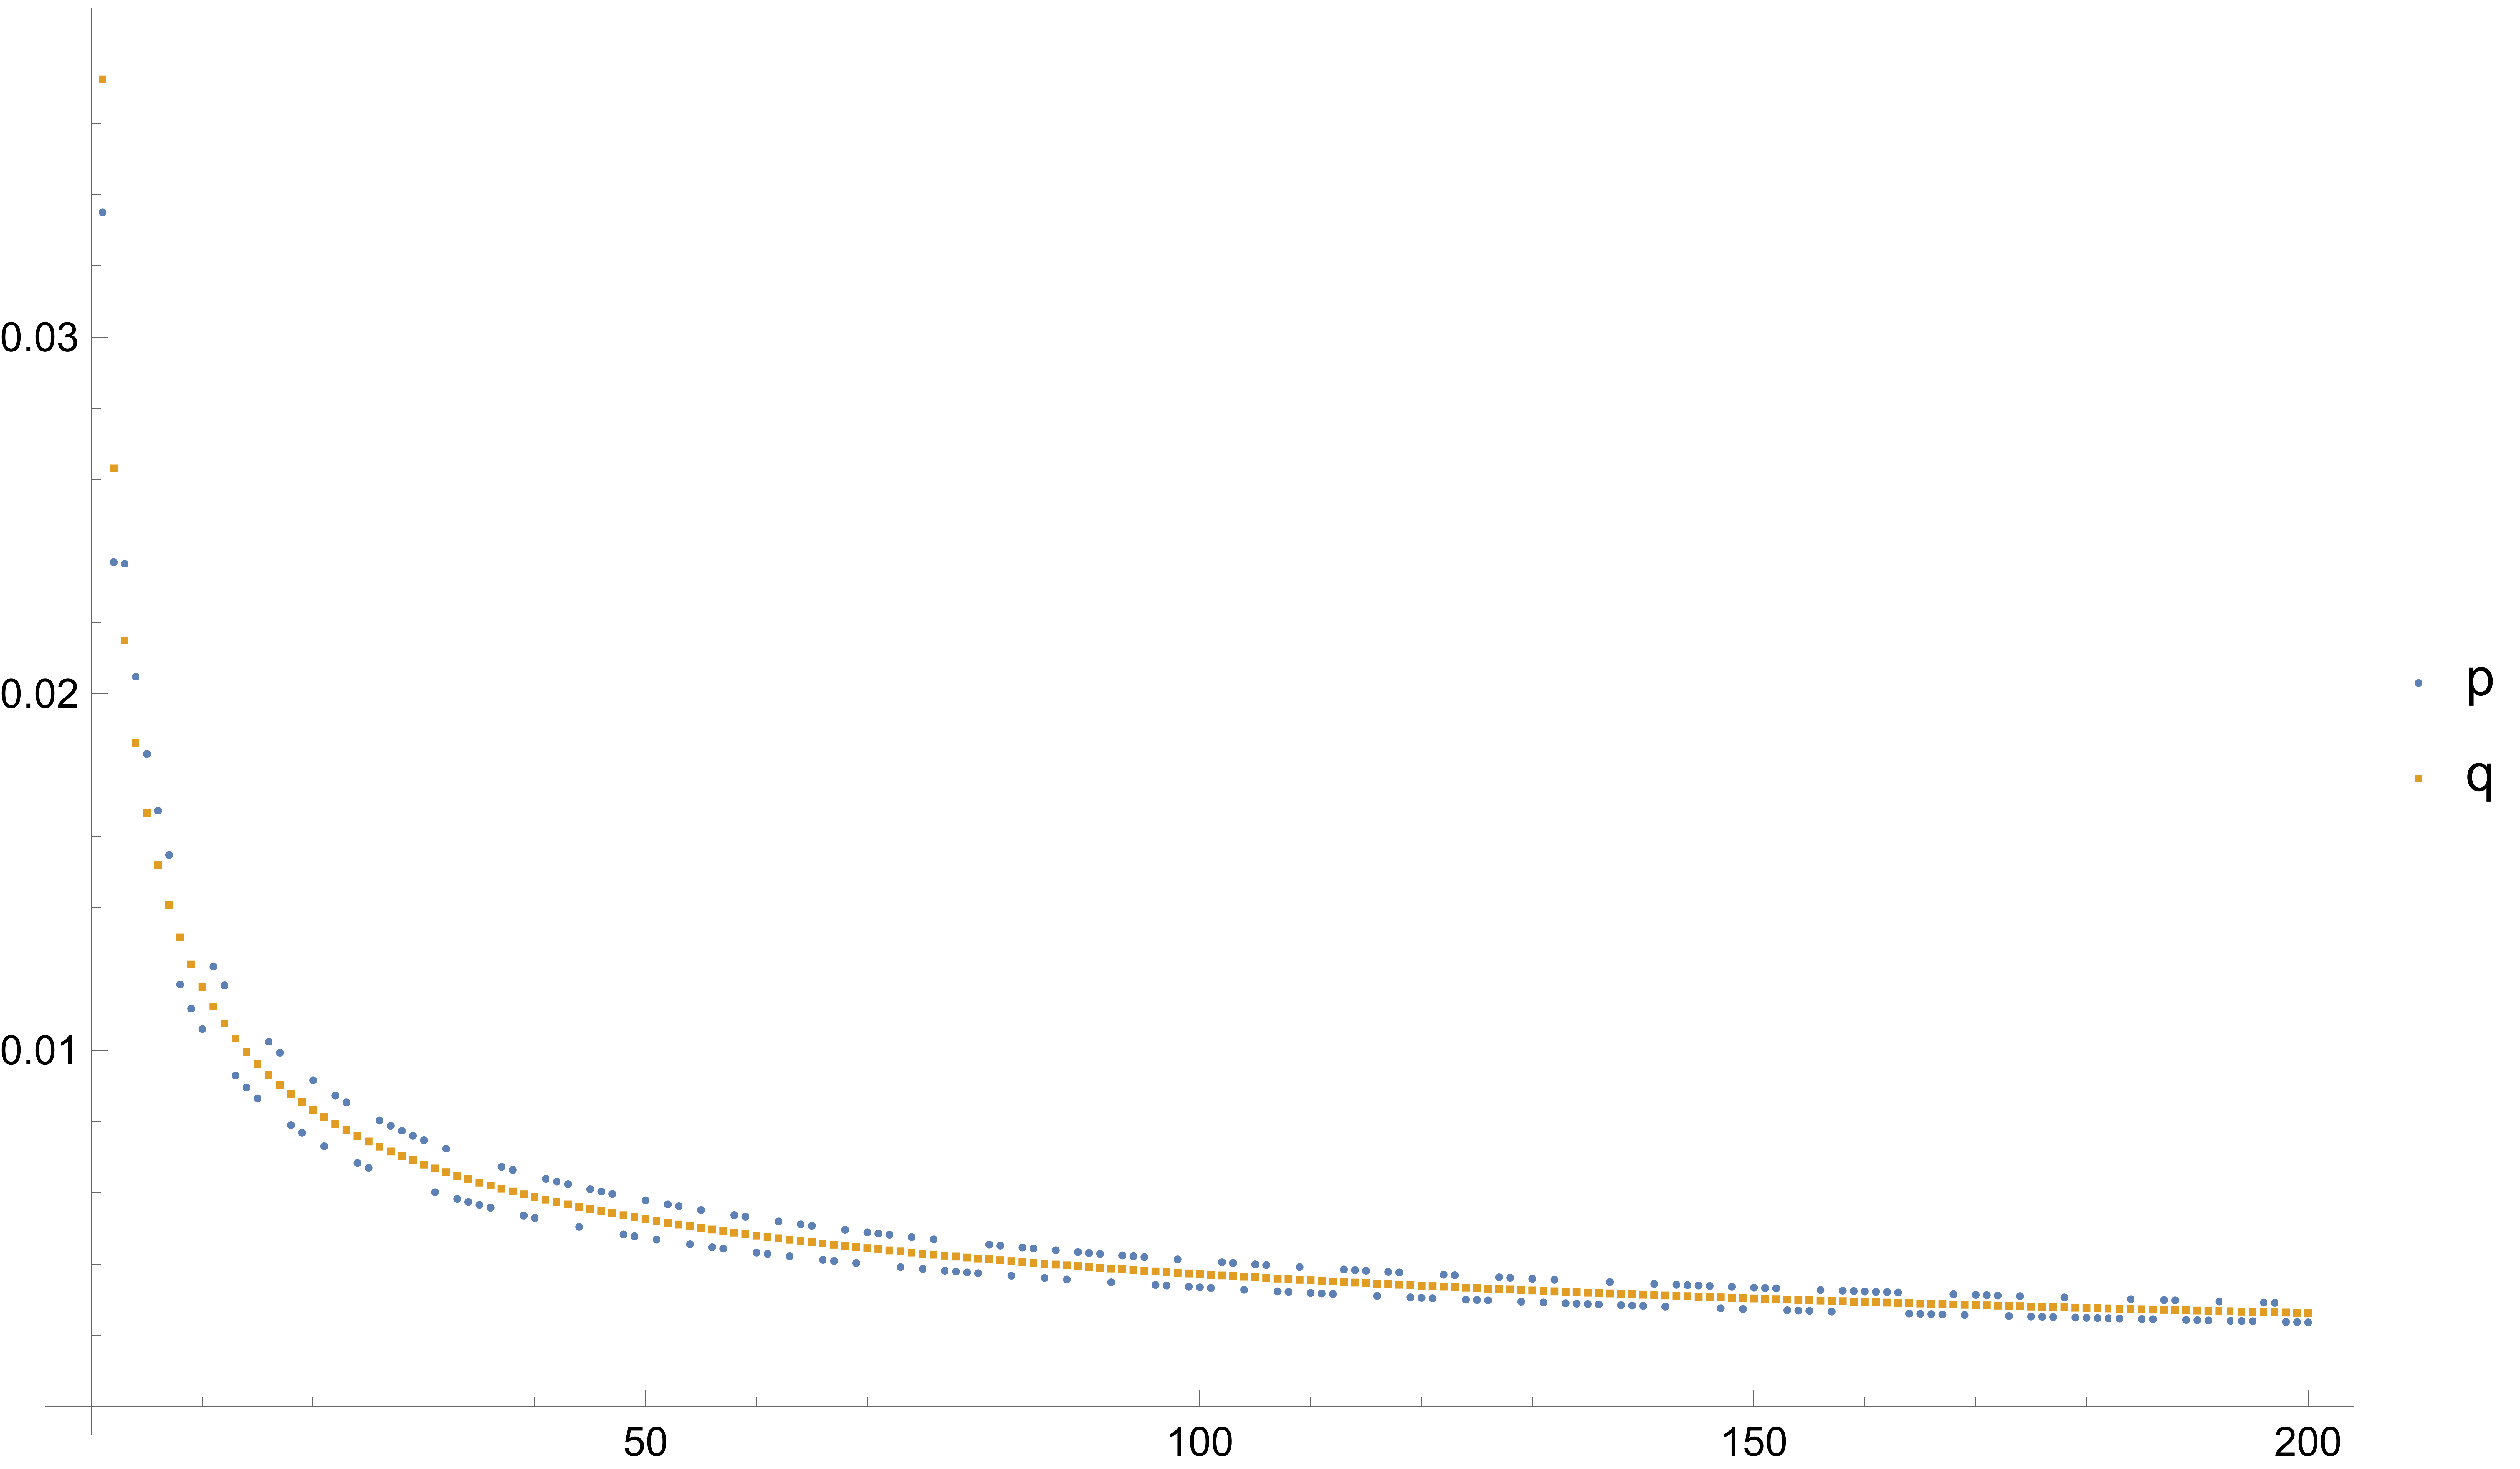
\includegraphics[width=1.0\textwidth]{figures/fig-lowerbound-zipf-pq}
	\caption{\label{fig:vv17:lb:zipf}Our reference $\q$ (Zipf distribution), along with a randomly chosen perturbation $\p$, here depicted for $\ab=200$, $\dst=1/10$.}
\end{figure}
%%%%%%%%%%%%%%%%%%%%%%%%%%%%%%%%%%%%%%%%%%%%%%%%%%%%%%%%%%%%%%%%%%%%%%%%%
While the second half (``tail'') of the distribution looks somewhat uniform (all probabilities between $\ab/2$ and $\ab$ are within a factor $\sqrt{2}$), the first half is clearly not, with the first few elements having much higher probability. Perturbing those heavy elements by the same relative amount as the rest, ``intuitively,'' is not a good idea, as it is easier to detect and can give away a lot more information. Instead, we will see what happens when we only perturb this somewhat-uniform tail of $\q$: define our $\alpha_i$'s by
\[
	\alpha_i \eqdef 
	\begin{cases}
		16\dst &\text{if } i \geq \frac{\ab}{2}\\
		0 &\text{ otherwise}
	\end{cases}
\]
In view of applying~\cref{theo:vv:lb}, we first check that the distance of our hard instances $\p_z$ to $\q$ will be at least $\dst$:
$
\max_{i} \alpha_i\q(i) = 16\dst\q(\ab/2) \ll \dst
$, and
\[
	\frac{1}{4}\sum_{i=1}^\ab \alpha_i\q(i) = 	\frac{4\dst}{H_{\ab,1/2}} \sum_{i=\frac{\ab}{2}}^\ab \frac{1}{\sqrt{i}} = 4\dst\Paren{1-\frac{H_{\frac{\ab}{2},1/2}}{H_{\ab,1/2}}} \geq 4\Paren{1-\frac{1}{\sqrt{2}}}\dst > \dst\,,
\]
so by~\cref{eq:vv:proba:far} the distance is fine. Turning to the sample complexity lower bound this will lead to, we compute
\[
	\sum_{i=1}^\ab \alpha_i^4 \q(i)^2 = \frac{(16\dst)^4}{H_{\frac{\ab}{2},1/2}^2}\sum_{i=\frac{\ab}{2}}^\ab \frac{1}{i} 
	= \frac{(16\dst)^4}{H_{\frac{\ab}{2},1/2}^2} \Paren{ H_{\ab} - H_{\frac{\ab}{2}} }
	\asymp \frac{\dst^4}{\ab}
\] 
since $H_{\ab} - H_{\ab/2} = \ln 2 + o(1)$. By~\cref{eq:vv:lb:samples}, this means we get a (tight) lower bound of $\Omega(\sqrt{\ab}/\dst^2)$ samples! All we needed to do was to restrict our perturbation to the ``near-uniform'' part of the reference distribution; crucially, this required the ability to choose different $\alpha_i$'s for different $i$, as allowed by~\cref{theo:vv:lb}.\medskip

To conclude this section, we will derive another corollary to~\cref{theo:vv:lb}, which provides the ``best'' perturbation possible for any given reference $\q$; that is, an optimal choice for the $\alpha_i$'s as a function of $\q$. Based on our previous example, we know that $\alpha_i$ somehow has to \emph{adapt} to $\q(i)$, to differentiate between the heavy elements and the ``near-uniform'' part of the distribution $\q$.

Now, on the one hand we want to establish as large a lower bound as possible, and so~\cref{eq:vv:lb:samples} says we should maximize
$
\sum_{i=1}^\ab \alpha_i^4\q(i)^2
$. On the other hand, for our lower bound to be meaningful, we also need our hard instances to be at distance $\dst$ from $\q$, and for that~\cref{eq:vv:proba:far} imposes the condition
$
\sum_{i=1}^\ab \alpha_i\q(i) \asymp \dst
$. Since
\begin{equation}
	\sum_{i=1}^\ab \alpha_i^4\q(i)^2 \leq \max_i \alpha_i^3\q(i) \cdot \sum_{i=1}^\ab \alpha_i\q(i)
\end{equation}
combining the two conditions leads us to try and maximize $\max_i \alpha_i^3\q(i)$, and the condition for equality in H\"older's inequality further suggests we should have $\alpha_i^3\q(i)$ constant; that is,
\begin{equation}
	\label{eq:vv:lb:intuition}
	\alpha_i \propto 1/\q(i)^{1/3}\,.
\end{equation}
We may not be able to do this exactly, as the theorem also requires that $\alpha_i \leq 1$, so we will have to cap our $\alpha_i$'s;  but this motivates the following idea. Without loss of generality, assume that $\q$ is non-increasing: $\q(1)\geq \q(2)\geq \dots\geq \q(\ab)$ (we can, since we know $\q$, and can permute the domain if we want) and $\dst\in(0,1/8]$; and assume, \emph{with} some loss of generality, that $\q(1)=\norminf{\q} \leq 1/2$. First, define $\alpha\geq 0$ as a value such that
\begin{equation}
	\label{eq:vv:lb:choice:alpha}
	\frac{1}{4}\sum_{i=2}^\ab \Paren{1\land \frac{\alpha}{\q(i)^{1/3}}}\q(i) = \dst
\end{equation}
where we start the summation at $i=2$ to (later) handle the (annoying) condition from~\cref{theo:vv:lb} on $\max_i \alpha_i\q(i)$, which will be $\alpha_1\q(1)$. To see why such a choice of $\alpha$ always exists, note that 
the LHS of~\cref{eq:vv:lb:choice:alpha} is continuous and non-decreasing in $\alpha$, equal to $0$ for $\alpha=0$, and goes to $\frac{1}{4}\sum_{i=2}^\ab \q(i) = \frac{1}{4}(1-\norminf{\q}) \geq \frac{1}{8}$ for $\alpha\to\infty$.

One we have this value $\alpha$, we can then set
\begin{equation}
	\label{eq:vv:lb:choice:alphai}
	\alpha_i =
	\begin{cases}
		1\land \frac{\alpha}{\q(i)^{1/3}} &\text{ if } 1\leq i\leq \ab\\
		\alpha_2\frac{\q(2)}{\q(1)} &\text{ if } i =1
	\end{cases}
\end{equation}
where the assumption that $\q$ is non-increasing implies that (i)~$\alpha_1\leq\alpha_2\leq \alpha_3\leq \dots \leq \alpha_\ab$, and (ii)~$\alpha_1\q(1)=\alpha_2\q(2)\geq \alpha_3\q(3)\geq \dots \geq \alpha_\ab\q(\ab)$ (since $\alpha_i\q(i) = \q(i)\land (\alpha\q(i)^{2/3})$).

\noindent Our (somewhat bizarre) choice of $\alpha_1$ is a technicality to ensure that
\[
	\max_i \alpha_i\q(i) = \alpha_1\q(1) = \frac{1}{2}(\alpha_1\q(1)+\alpha_2\q(2)) \leq \frac{1}{2}\sum_{i=1}^\ab \alpha_i\q(i)
\]
so that the condition of~\cref{theo:vv:lb} preceding~\cref{eq:vv:proba:far} is satisfied. Letting $L$ to be the largest value $i\geq 2$ such that $\alpha\q(i)^{-1/3} \leq 1$, we then can rewrite~\cref{eq:vv:lb:choice:alpha} as
\begin{equation}
	\label{eq:vv:lb:choice:alpha:2}
	\alpha\sum_{i=2}^L \q(i)^{2/3} + \sum_{i=L+1}^\ab \q(i) = 4\dst\,,
\end{equation}
from which $\alpha \leq 4\dst/\sum_{i=2}^L \q(i)^{2/3}$. Finally, recalling~\cref{eq:vv:lb:samples}, we bound
\begin{align}
	\sum_{i=1}^\ab \alpha_i^4\q(i)^2
	&\leq \sum_{i=2}^\ab \alpha_i^4\q(i)^2
	= \alpha^4\sum_{i=2}^L \q(i)^{2/3} + \sum_{i=L+1}^\ab \q(i)^2 \notag\\
	&\leq \alpha^3\Paren{\alpha\sum_{i=2}^L \q(i)^{2/3} + \sum_{i=L+1}^\ab \q(i) } \notag\\
	&= 4\dst \alpha^3 \tag{By~\cref{eq:vv:lb:choice:alpha:2}}\\
	&\leq \frac{(4\dst)^4}{\Paren{\sum_{i=2}^L \q(i)^{2/3}}^3}
\end{align}
where we used that $\q(i) \leq \alpha^3$ for all $i \geq L+1$ in the second inequality. Applying~\cref{theo:vv:lb} (along with the similar arguments as in the proof of~\cref{theo:uniformity:lb:vv}), what this shows is a lower bound of
\begin{equation}
	\label{eq:vv:lb:complicated}
	\bigOmega{ \frac{\Paren{\sum_{i=2}^L \q(i)^{2/3}}^{3/2}}{\dst^2}}
\end{equation}
samples to test identity to $\q$, where $L=L(\q,\dst)$ is defined above, and $\q$ satisfies $\norminf{\q}\leq 1/2$ and is (without loss of generality) assumed non-decreasing. This bound can seem quite daunting, due to the way $L(\q,\dst)$ is defined; fortunately, we can relax it a little to make it more interpretable (though technically looser). 

Observe that~\cref{eq:vv:lb:choice:alpha:2} also implies $\sum_{i=L+1}^\ab \q(i) \leq 4\dst$; thus, if we define $K=K(\q,\dst)$ as the largest integer such that $\sum_{i=K}^\ab \q(i) > 4\dst$, we are guaranteed that $K(\q,\dst)\leq L(\q,\dst)$ and therefore $\sum_{i=2}^K \q(i)^{2/3} \leq \sum_{i=2}^L \q(i)^{2/3}$. This leads to the following corollary:
\begin{theorem}
  \label{theo:2/3:lb:vv}
Given a probability distribution $\q\in\distribs{\ab}$, let $\tilde{\q}^{-\!\max}_{-4\dst}$ denote the vector obtained by seeing $\q$ as a vector in $[0,1]^\ab$, and removing (i)~its largest entry, and (ii)~its smallest entries, stopping just before the total removed exceeds $4\dst$. Then every testing algorithm for identity with reference $\q$ must have sample complexity $\ns(\ab,\dst,1/3) = \Omega(\lVert\tilde{\q}^{-\!\max}_{-4\dst}\rVert_{2/3}/\dst^2)$, provided that $\norminf{\q}\leq 1/2$ and $\dst\in(0,1/8]$.
\end{theorem}
\noindent One can check that this does retrieve the $\Omega(\sqrt{\ab}/\dst^2)$ testing lower bound both when (1)~$\q$ is the uniform distribution, (2)~$\q$ is the Zipf  distribution we saw in our earlier example\medskip.\exercise{Check it!\cref{???}}

%%%% Comment on uses beyond identity testing! E.g., LB for other problems.

Finally, it is worth mentioning that~\cref{theo:vv:lb} is not restricted to identity testing (although this is the application we detailed in this section). One can use it to establish indistinguishability results for other questions, focusing on the sample complexity lower bound it provides (\cref{eq:vv:lb:samples}) and possibly ignoring the distance part (\cref{eq:vv:proba:far}). For instance, it can be used to establish sample complexity lower bounds for testing in other norms than total variation distance, or to obtain lower bounds on estimating some parameter of interest.

%%%%%%%%%%%%%%%%%%%%%%%%%%%%%%%%%%%%%%%%%%%%%%%%%%%
\section{Proving hardness by reductions}
	\label{ssec:lb:reductions}
In this section, we will shift focus a little, and discuss how to \emph{leverage work (other) people did} in order to establish new sample complexity lower bounds. To illustrate the idea, consider the property $\property^{\searrow}=\cup_{\ab=1}^\infty \property^{\searrow}_\ab$ of \emph{monotone} (non-increasing) distributions,
\ie
\begin{equation}
\property^{\searrow}_\ab \eqdef \setOfSuchThat{ \p\in\distribs{\ab} }{ \p(1)\geq \p(2) \geq \dots \geq \p(\ab) }
\end{equation}
Say we want to test this property $\property^{\searrow}$: that is, given samples from a distribution over $\{1,2,\dots,\ab\}$, we want to test whether its pmf is non-increasing; more specifically, say we want to show it is not easy. We could try to use techniques from the previous subsections (though probably not directly those from~\cref{ssec:momentmatching}, as $\property^{\searrow}$ is most definitely not a symmetric property) to establish a sample complexity lower bound: this will require quite a bit of thinking and at least of few non-trivial computations.

But we have already shown (in a few different ways by now) that \emph{uniformity} testing had sample complexity $\Omega(\sqrt{\ab}/\dst^2)$. Can we somehow show that testing monotonicity is \emph{at least as hard}, and get the same lower bound without working much more? Enters the concept of \emph{reduction}, quite central to (theoretical) computer science. We already saw it in~\cref{ssec:l1:reduction}, when we used it to show how to use any uniformity testing algorithm for the more general problem of identity testing: that is, we described a reduction from uniformity to identity testing to get an algorithm (upper bound) for the latter, using an algorithm for the former. But every coin has two sides, and a reduction can be used to show lower bounds too!

Here's how. Imagine we had an ``efficient'' reduction from uniformity testing to monotonicity testing: given samples from an arbitrary distribution $\p\in\distribs{\ab}$, we can obtain samples from a distribution $\Phi(\p)\in\distribs{\ab'}$ such that (i)~$\Phi(\p)\in\property^{\searrow}_{\ab'}$ whenever $\p=\uniform_\ab$, and $\totalvardist{\Phi(\p)}{\property^{\searrow}_{\ab'}} > \dst'$ whenever $\totalvardist{\p}{\uniform_\ab} > \dst$. We allow the domain to change a little, from $\ab$ to some (not much larger) $\ab'$; and similarly for the distance parameter, originally $\dst$, which can become some other (not much smaller) value $\dst'$. See~\cref{fig:reduction:monotonicity} for a depiction.

\begin{figure}[htbp]\centering
\tikzset {_3eubqr20l/.code = {\pgfsetadditionalshadetransform{ \pgftransformshift{\pgfpoint{0 bp } { 0 bp }  }  \pgftransformrotate{0 }  \pgftransformscale{2.64 }  }}}
\pgfdeclarehorizontalshading{_y5uoy9rpz}{150bp}{rgb(0bp)=(0.99,0.97,0.93);
rgb(54.285714285714285bp)=(0.99,0.97,0.93);
rgb(61.96428571428571bp)=(0.98,0.95,0.95);
rgb(100bp)=(0.98,0.95,0.95)}
\tikzset{every picture/.style={line width=0.75pt}} %set default line width to 0.75pt        

\begin{tikzpicture}[x=0.75pt,y=0.75pt,yscale=-1.3,xscale=1.3]
%uncomment if require: \path (0,300); %set diagram left start at 0, and has height of 300

%Shape: Polygon Curved [id:ds24835565753561872] 
\draw  [xshift=-100pt,draw opacity=0.05,scale=0.85,yshift=20pt,xshift=-20pt][shading=_y5uoy9rpz,_3eubqr20l] (228.87,88.88) .. controls (266.87,64.88) and (266.87,111.88) .. (282.87,123.88) .. controls (298.87,135.88) and (360.87,96.88) .. (335.87,141.88) .. controls (310.87,186.88) and (389.87,249.88) .. (305.87,226.88) .. controls (221.87,203.88) and (251.87,247.88) .. (208.87,236.88) .. controls (165.87,225.88) and (201.87,193.88) .. (183.87,172.88) .. controls (165.87,151.88) and (157.87,118.88) .. (191.87,123.88) .. controls (225.87,128.88) and (190.87,112.88) .. (228.87,88.88) -- cycle ;
%Shape: Circle [id:dp2977666721327956] 
\draw  [draw opacity=0,scale=0.45,xshift=-91pt,yshift=153pt][fill={rgb, 255:red, 253; green, 170; blue, 30 }, fill opacity=0.7 ][general shadow={fill={rgb, 255:red, 245; green, 166; blue, 35 },shadow xshift=0pt,shadow yshift=0pt, opacity=0 }] (242,165.5) .. controls (248,147) and (253,132) .. (271.5,132) .. controls (290,132) and (305,147) .. (308,165.5) .. controls (310,184) and (290,199) .. (271.5,199) .. controls (253,199) and (238,184) .. (242,165.5) -- cycle ;
%Shape: Circle [id:dp2977666721327956] 
\draw  [draw opacity=0.05,scale=0.25,xshift=0pt,yshift=375pt][fill={rgb, 255:red, 253; green, 170; blue, 30 }, fill opacity=0.99 ][general shadow={fill={rgb, 255:red, 245; green, 166; blue, 35 },shadow xshift=0pt,shadow yshift=0pt, opacity=0 }] (242,165.5) .. controls (248,147) and (253,132) .. (271.5,132) .. controls (290,132) and (305,147) .. (308,165.5) .. controls (310,184) and (290,199) .. (271.5,199) .. controls (253,199) and (238,184) .. (242,165.5) -- cycle ;
%Shape: Ellipse [id:dp5805520465941827] 
\node at (50,120) (nodedistribs) {$\distribs{\ab}$};
\node at (90,145) (nodefar) {};
\node at (60,175) (nodeeps) {\scriptsize$\dst$};
\node at (70,168) (nodepropertyunif) {$\uniform_{\ab}$};
\node at (65,168) (nodepropertyunifstartarrow) {};

%%%%%%%%%%%%%%%%%%%%%%%%%%%%%%%%%%%%%%%%%%%%%%%%%%%%%%%%%%%%%%%%%%%%


%Shape: Polygon Curved [id:ds24835565753561872] 
\draw  [draw opacity=0.05][shading=_y5uoy9rpz,_3eubqr20l] (228.87,88.88) .. controls (266.87,64.88) and (266.87,111.88) .. (282.87,123.88) .. controls (298.87,135.88) and (360.87,96.88) .. (335.87,141.88) .. controls (310.87,186.88) and (389.87,249.88) .. (305.87,226.88) .. controls (221.87,203.88) and (251.87,247.88) .. (208.87,236.88) .. controls (165.87,225.88) and (201.87,193.88) .. (183.87,172.88) .. controls (165.87,151.88) and (157.87,118.88) .. (191.87,123.88) .. controls (225.87,128.88) and (190.87,112.88) .. (228.87,88.88) -- cycle ;
%Shape: Circle [id:dp2977666721327956] 
\draw  [draw opacity=0][fill={rgb, 255:red, 253; green, 170; blue, 30 }  ,fill opacity=0.70 ][general shadow={fill={rgb, 255:red, 245; green, 166; blue, 35 },shadow xshift=0pt,shadow yshift=0pt, opacity=0 }] (242,165.5) .. controls (248,147) and (253,132) .. (271.5,132) .. controls (290,132) and (305,147) .. (308,165.5) .. controls (310,184) and (290,199) .. (271.5,199) .. controls (253,199) and (238,184) .. (242,165.5) -- cycle ;
%Shape: Circle [id:dp2977666721327956] 
\draw  [draw opacity=0.05, scale=0.8,xshift=51pt,yshift=31pt][fill={rgb, 255:red, 253; green, 170; blue, 30 }  ,fill opacity=0.99 ][general shadow={fill={rgb, 255:red, 245; green, 166; blue, 35 },shadow xshift=0pt,shadow yshift=0pt, opacity=0 }] (242,165.5) .. controls (248,147) and (253,132) .. (271.5,132) .. controls (290,132) and (305,147) .. (308,165.5) .. controls (310,184) and (290,199) .. (271.5,199) .. controls (253,199) and (238,184) .. (242,165.5) -- cycle ;
%Shape: Ellipse [id:dp5805520465941827] 
\node at (240,120) (nodedistribsprime) {$\distribs{\ab'}$};
\node at (220,170) (nodefarprime) {};
\node at (245,175) (nodeepsprime) {\scriptsize$\dst'$};
\node at (275,165) (nodeproperty) {$\property^{\searrow}_{\ab'}$};



\draw [dotted,->] (nodefar) to  [out=-25,in=225] (nodefarprime);
\draw [dotted,->] (nodepropertyunifstartarrow) to [out=45,in=100] (nodeproperty);
\end{tikzpicture}
\caption{Illustration of what a reduction from uniformity testing to monotonicity testing is. The uniform distribution is mapped to some monotone distribution, while distributions far from uniform are mapped to distributions far from monotone. (Things that are neither uniform nor far from it can be mapped to anything.)\label{fig:reduction:monotonicity}}
\end{figure}
\noindent Then, any algorithm $\Tester$ for testing $\property^{\searrow}$ (with parameters $\ab',\dst'$) can be used to test uniformity (with parameters $\ab,\dst$): convert the samples from $\p\in\distribs{\ab}$ to samples from $\Phi(\p)\in\distribs{\ab'}$, run $\Tester$ on them, and output what this tester returns. Which is great\dots except that we know that $\Omega(\sqrt{\ab}/\dst^2)$ samples are required for the latter task; so the sample complexity $\ns$ of $\Tester$ must satisfy $\ns(\ab',\dst',1/3) = \Omega(\sqrt{\ab}/\dst^2)$. We get a lower bound! Whose meaningfulness, of course, depends a lot on how $\ab'$ and $\dst'$ are related to $\ab$ and $\dst$.\smallskip

Let us look at an example, to make things more concrete. Consider the following (randomized) mapping $\Psi\colon[\ab]\to[2\ab]$: 
\begin{description}
	\item[$\Psi$:] Given $i \in [\ab]$, return $i$ with probability $\frac{1}{2}$ and $\ab+i$ otherwise.
\end{description}
Applying this to a sample from a probability distribution $\p\in\distribs{\ab}$ results in a sample from $\Phi(\p)$ over $\ab'\eqdef2\ab$ (where $\Phi\colon\distribs{\ab}\to\distribs{\ab'}$), given by
\begin{equation}
	\label{eq:reduction:monotonicity}
	\Phi(\p)(i) = \frac{1}{2}\p(i\bmod\ab)
\end{equation}
which ``duplicates the domain and puts two contiguous copies of $\p$ next to each other.'' Why is it a good thing to consider? For a start, if we apply this to the uniform distribution $\uniform_\ab$, we end up with $\Phi(\uniform_\ab) = \uniform_{2\ab}$, the uniform distribution on our new domain, which is definitely in $\property^{\searrow}_{2\ab}$ (the uniform distribution may not be the most interesting monotone distribution, but it is a monotone distribution nonetheless). So this fits at least half the bill: as you will show in~\cref{ex:reduction:monotone},\exercise{Show this.} it also fits the other half: distributions which are $\dst$-far from uniform are mapped to distributions $\dst'$-far from uniform, where $\dst'\eqdef \dst/2$.

\begin{figure}[htbp]\centering
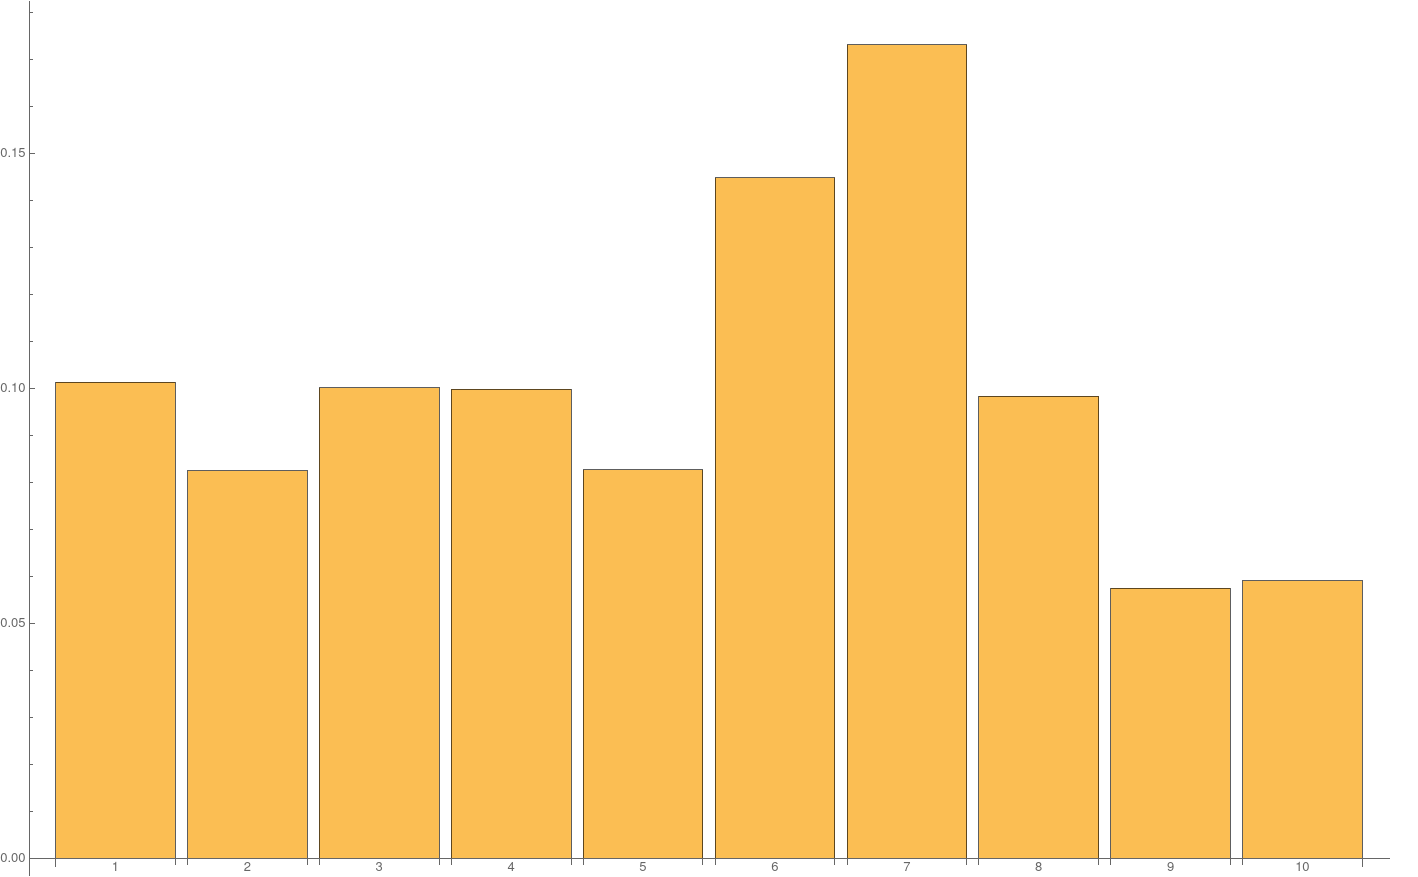
\includegraphics[width=.45\textwidth]{figures/fig-reduction-uniformity}\hfill
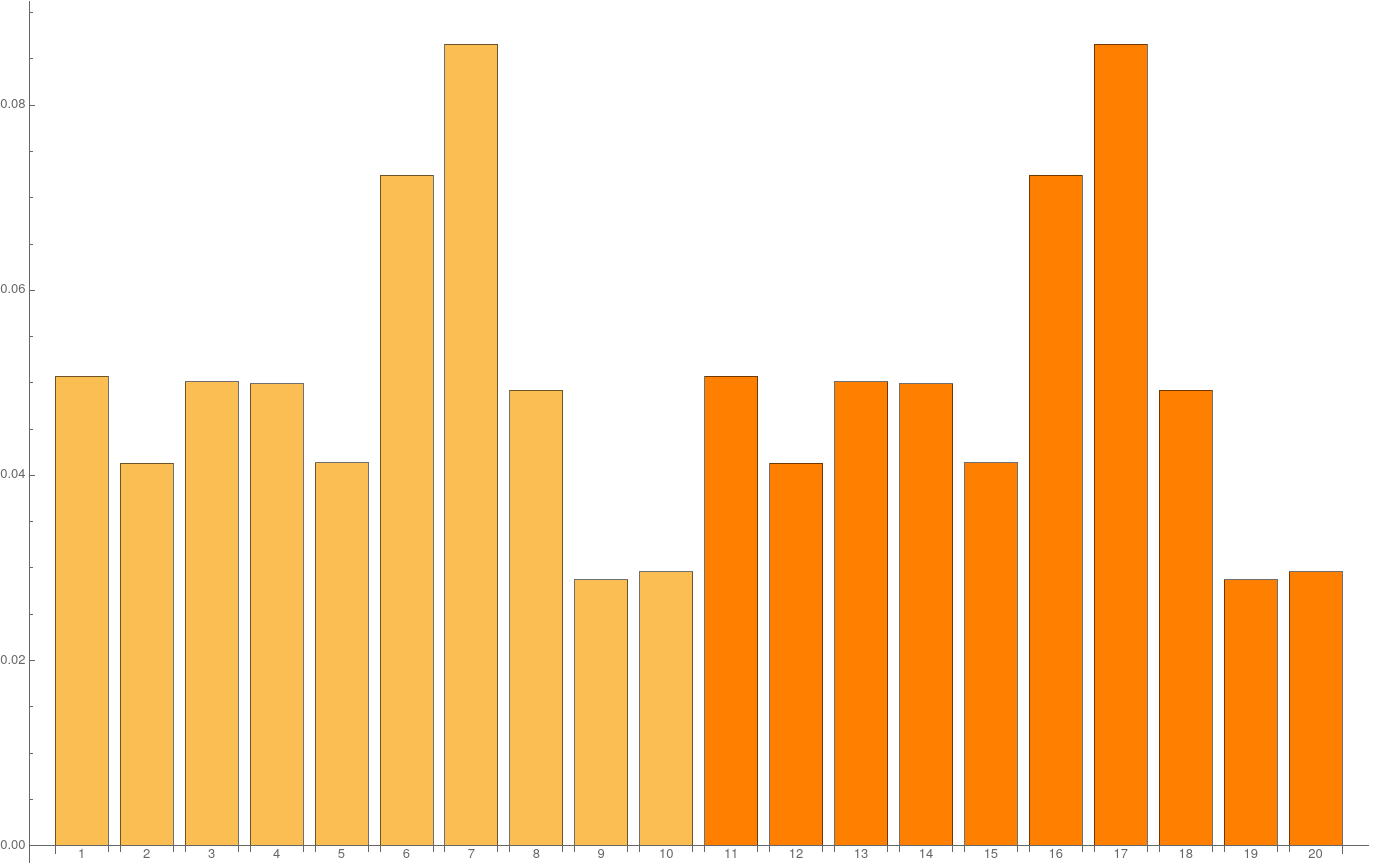
\includegraphics[width=.45\textwidth]{figures/fig-reduction-uniformity2}
\caption{An example of the reduction outlined above, with a distribution $\p$ over a domain of size $\ab=20$ (left) and the resulting $\Phi(\p)$ on a domain of size $\ab'=2\ab=40$ on the right.\label{fig:reduction:monotonicity:example}}
\end{figure}
By the above discussion, the lower bound on uniformity testing directly implies that monotonicity testing with parameters $2\ab$ and $\dst/2$ must have sample complexity $\Omega(\sqrt{\ab}/\dst^2)$. Since constant factors are just constant factors, this leads to the following:
\begin{theorem}
	\label{theo:lb:testing:monotonicity}
Every testing algorithm for $\property^{\searrow}$ (monotonicity) must have sample complexity $\ns(\ab,\dst,1/3) = \Omega(\sqrt{\ab}/\dst^2)$.
\end{theorem}
\noindent(As a side note, this is known to be tight, as least for $\dst \gg \sqrt{\log\ab}/\ab^{1/4}$.) Crucially, reductions comes with another advantage: if we were to introduce another parameter (focusing on the dependence on $\errprob$, for instance), or work with constrained measurements as in~\cref{chap:constrained}, then as long as our reduction goes through in the setting considered, we only need to derive the uniformity testing lower bound in that setting to immediately get the corresponding lower bound for monotonicity testing as well. As said earlier, reductions are great to avoid unnecessary work!

\paragraph{A general result.} The above reduction was quite specific to monotonicity testing: ideally, we would like more general statements, allowing us to derive as many lower bounds as possible while having to think as little as possible. In the rest of this section, we are going to describe such a result, which can be seen as some converse to the ``testing-by-learning'' baseline from~\cref{lemma:learning:baseline}. The high-level idea is as follows: suppose we have two properties $\property' \subseteq \property$, and we know that $\property'$ is hard to test. Then we want to conclude that $\property$, too, is hard to test~--~at least as hard as $\property'$. (In our earlier example, $\property'$ was uniformity, and $\property$ monotonicity: since the uniform distribution is monotone, the inclusion indeed holds.)

The issue with this conclusion, however, \emph{is that it is not true.} One can come up with very simple examples showing it: taking $\property_\ab = \distribs{\ab}$, for example (the trivial property containing all discrete distributions) and $\property'_\ab=\{\uniform_\ab\}$, we clearly have $\property'_\ab \subseteq \property_\ab$, yet $\property_\ab$ can be tested with exactly 0 samples~--~while $\property'_\ab$ requires $\Omega(\sqrt{\ab}/\dst^2)$.

Still, in that counterexample, the property $\property$ itself is ginormous (all distributions!), which somewhat explains the issue: in contrast, the property $\property^{\searrow}$ of monotone distributions was much smaller. If we restrict the statement to ``simple enough'' properties, then maybe the statement will hold? \textit{E.g.}, what about properties which can be \emph{learned} efficiently?  
As we will see momentarily, this is indeed the case, albeit for a very specific sense of ``learning'' we first need to introduce.

\begin{definition}[Agnostic learning]
	A class $\class=\bigcup_{\ab=1}^\infty \class_\ab$ is said to be \emph{agnostically learnable} with sample complexity $\ns(\ab,\dst,\errprob)$ if there is an algorithm which, given $\ns=\ns(\ab,\dst,\errprob)$ \iid samples from an unknown \emph{arbitrary} distribution $\p\in\distribs{\ab}$, outputs a distribution $\hat{\p}$ such that
	\[
		\totalvardist{\p}{\hat{\p}} \leq C\cdot \inf_{\q\in\class_\ab} \totalvardist{\p}{\q} + \dst
	\]
with probability at least $1-\delta$, where $C\geq 1$ is an absolute constant.
\end{definition}
In other terms, an agnostic learning algorithm works even in the unrealizable setting (when $\p\notin\class_\ab$), and its output is ``nearly as good'' as the best candidate from $\class_\ab$ would be. The main result of this section is the following theorem, which roughly states that ``if a property is easy to learn, then it is as hard to test as its hardest sub-property:''
\begin{theorem}[Hardness by Reduction]\label{theo:hardness:subclass}
  Fix any property $\property$, and suppose there exists $\property'\subseteq \property$ such that the following holds.
  \begin{enumerate}
    \item\label{theo:hardness:subclass:item1} Agnostic learning of $\property$ (with a given ``agnostic constant'' $C\geq 1$) has sample complexity at most $\ns_{\mathcal{L}}(\ab,\dst,\delta)$;
    \item\label{theo:hardness:subclass:item2} Testing $\property'$ has sample complexity at least $\ns_{\mathcal{T}}(\ab,\dst,\errprob)$;
    \item\label{theo:hardness:subclass:item3} There exists a range of parameters $\ab,\dst,\errprob$ for which learning $\property$ is easier than testing $\property'$: 
    	\[
    		\ns_{\mathcal{L}}(\ab,C\dst,\errprob) \leq \frac{1}{2}\ns_{\mathcal{T}}(\ab,3C\dst,2\errprob)
    	\]
  \end{enumerate}
  Then, for $\ab,\dst,\errprob$ in that range of parameters, every testing algorithm for $\property$ must have sample complexity at least $\frac{1}{2}\ns_{\mathcal{T}}(\ab,3C\dst,2\errprob)$.
\end{theorem}
\begin{proof}
The idea of the proof is quite simple: suppose we have a testing algorithm $\Algo$ for $\property$ with sample complexity $\ns_\Algo(\ab,\dst,\errprob)$, and let $\Learner$ be the agnostic learning algorithm for $\property$ with sample complexity $\ns_{\mathcal{L}}(\ab,\dst,\errprob)$ promised by~\cref{theo:hardness:subclass:item1}. Then we can combine both to obtain a testing algorithm for $\property'$: but since $\property'$ is hard to test, this testing algorithm cannot be \emph{too} sample-efficient (it must take at least $\ns_{\mathcal{T}}$ samples), giving us a lower bound $\ns_\Algo+\ns_\Learner \geq \ns_{\mathcal{T}}$. (Note that we only care about sample complexity, and do not make any assumption on computational efficiency.)

\noindent In more detail, consider the following testing algorithm $\Algo'$ for $\property'$: on input $\ab,\dst,\errprob$,
\begin{itemize}
	\item Run $\Algo$ with parameters $\ab,\dst/(3C),\errprob/2$; let $b\in\{\reject,\accept\}$ be the result.
	\item Run $\Learner$ with parameters $\ab,\dst/3,\errprob/2$; let $\hat{\p}$ be the output.
	\item Check whether $\totalvardist{\hat{\p}}{\property'} \leq \dst/3$; let $b'\in\{\reject,\accept\}$ indicate the result (this is purely computational and requires no samples from $\p$).
	\item Return $b\land b'$ (\ie \accept if, and only if, both $b$ and $b'$ were \accept).
\end{itemize}
Since both $\Algo$ and $\Learner$ were run with error probability $\errprob/2$, by a union bound they are simultaneously correct with probability at least $1-\errprob$. Assume hereafter this event holds.
\begin{itemize}
\item If $\p\in\property'$, then \textit{a fortiori} $\p\in\property$, and $\Algo$ returns $b=\accept$. Moreover, $\totalvardist{\p}{\hat{\p}} \leq C\cdot 0 + \dst/3 = \dst/3$, so $b'=\accept$ as well, and overall $\Algo'$ returns \accept.
\item Let us now argue the ``soundness.'' Suppose that $\Tester'$ returns $\accept$: this means that $b=\accept$, and so since $\Algo$ is a testing algorithm for $\property$ we must have $\totalvardist{\p}{\property} \leq \dst/(3C)$. But then, since $\Learner$ is an agnostic learner for $\property$, we get $\totalvardist{\p}{\hat{\p}} \leq C\cdot \totalvardist{\p}{\property} + \dst/3 \leq 2\dst/3$. And finally, since the last check was successful as well ($b'=\accept$), we have that $\totalvardist{\hat{\p}}{\property'} \leq \dst/3$. By the triangle inequality, it follows that
\[
	\totalvardist{\p}{\property'} \leq \totalvardist{\p}{\hat{\p}}+\totalvardist{\hat{\p}}{\property'} \leq \dst\,.
\]
By contrapositive, if $\totalvardist{\p}{\property'} > \dst$ then it must be the case that $\Tester'$ returns $\reject$.
\end{itemize}
So $\Tester'$ is a \textit{bona fide} testing algorithm for $\property'$, and its sample complexity is
\[
	\ns'(\ab,\dst,\errprob) = \ns_\Algo(\ab,\dst/(3C),\errprob/2) + \ns_{\mathcal{L}}(\ab,\dst/3,\errprob/2)
\]
or, reparameterizing, 
\[
	\ns'(\ab,3C\dst,2\errprob) = \ns_\Algo(\ab,\dst,\errprob) + \ns_{\mathcal{L}}(\ab,C\dst,\errprob)\,.
\]
But since we know by~\cref{theo:hardness:subclass:item2} that $\property'$ is hard to test, we must then have
\[
	\ns_\Algo(\ab,\dst,\errprob) + \ns_{\mathcal{L}}(\ab,C\dst,\errprob) \geq \ns_{\mathcal{T}}(\ab,3C\dst,2\errprob)
\]
which by~\cref{theo:hardness:subclass:item3} implies $\ns_\Algo(\ab,\dst,\errprob) \geq \ns_{\mathcal{T}}(\ab,3C\dst,2\errprob)$, and proves the theorem.
\end{proof}

With this theorem in hand, proving a sample complexity lower bound for a given property $\property$ boils down to scouring the literature to check if (1)~$\property$ is easy to learn, and (2)~something (anything!) inside $\property$ is known to be hard to test. Note that the result may not always be an \emph{optimal} lower bound; but it often gets quite close to it, and is a simple and valuable starting point.\smallskip

To conclude, let us see a direct application of this theorem to the property $\property^{\searrow}$. We can use the fact that monotone distributions can be agnostically learned with $O(\log(1+\dst\ab)/\dst^3)$ samples~\citep{Birge87,DDS:12} along with our uniformity testing lower bound (taking $\property'_\ab \eqdef \{\uniform_\ab\}$). This lets us derive the same $\Omega(\sqrt{\ab}/\dst^2)$ sample complexity lower bound for testing $\property^{\searrow}$ as in~\cref{theo:lb:testing:monotonicity}, with the additional (small) restriction $\dst \gg (\log\ab)/\sqrt{\ab}$. Here again, we relied on the uniformity testing lower bound: it is worth pointing out that we can (and sometimes must) use other ``hard-to-test'' sub-properties than uniformity! We will see such an example in~\cref{ex:testing:pbd}, where you will be asked to prove a lower bound on testing ``Poisson Binomial Distributions.''

% Exercise VV17 for Binomial + this -> LB for PBDs
%%%%%%%%%%%%%%%%%%%%%%%%%%%%%%%%%%%%%%%%%%%%%%%%%%%
%%\section{Application: distributed inference}

%%%%%%%%%%%%%%%%%%%%%%%%%%%%%%%%%%%%%%%%%%%%%%%%%%%
\section{Historical notes}
\tbc
\citet{BlaisCG17} for another type of reductions (via communication complexity)

%%%%%%%%%%%%%%%%%%%%%%%%%%%%%%%%%%%%%%%%%%%%%%%%%%%%%%%%%%%%%%%%%%%%%%%%%
%%%%%%%%%%%%%%%%%%%%%%%%%%%%%%%%%%%%%%%%%%%%%%%%%%%%%%%%%%%%%%%%%%%%%%%%%
\section{Exercises}
\begin{question}[$\star$]\label{ex:reduction:monotone}
  Prove that the mapping $\Phi$ defined in~\cref{eq:reduction:monotonicity} does satisfy the requirements of a reduction, for $\ab'=2\ab$ and $\dst'=\dst/2$. That is, if $\p\in\distribs{\ab}$ is $\dst$-far from $\uniform_\ab$, then $\Phi(\p)\in\distribs{2\ab}$ is $\dst'$-far from every distribution $\q\in\property^{\searrow}_{2\ab}$. \textit{(Hint: for any given monotone $\q$, analyse the distance $\totalvardist{\Phi(\p)}{\q}$ according to whether $\q(\ab) > 1/(2\ab)$ or not, relating this to the set $S\subseteq[\ab]$ on which $\p$ is greater than $\uniform_\ab$.)} Moreover, show that this loss by a factor $1/2$ in the distance is necessary.
\end{question}
\iffalse %%%%%%%%%%% Hide answer
\begin{proof}[Solution of~\cref{ex:reduction:monotone}]
Fix any $\p\in\distribs{\ab}$ such that $\totalvardist{\p}{\uniform_\ab}>\dst$, and let $S\subseteq [\ab]$ the set which witnesses it:
$S\eqdef \setOfSuchThat{ 1\leq i\leq \ab }{\p(i)> 1/\ab }$ 
which satisfies 
\[
	\p(S)-\uniform_\ab(S) = \uniform_\ab([\ab]\setminus S)- \p([\ab]\setminus S) >\dst
\]
Further define $T \eqdef [\ab]\setminus S \subseteq \{1,2,\dots,\ab\}$, and $S+\ab = \setOfSuchThat{i+\ab}{i\in S} \subseteq \{\ab+1,\dots,2\ab\}$. 
By definition of $\Phi(\p)$, we then have
\[
	\uniform_{2\ab}(T)-\Phi(\p)(T)=\Phi(\p)(S+\ab)-\uniform_{2\ab}(S+\ab)= \frac{1}{2}(\p(S)-\uniform_\ab(S)>\frac{\dst}{2}\,.
\]
Now, fix any monotone distribution $\q\in\property^{\searrow}_{2\ab}$. We have two cases:
\begin{itemize}
\item If $\q(\ab) > 1/(2\ab)$, then, since $\q$ is monotone, $\q(i) > 1/(2\ab)$ for every $i \leq \ab$. This implies
\[
	\q(T)-\Phi(\p)(T) \geq \uniform_{2\ab}(T)-\Phi(\p)(T) > \frac{\dst}{2}
\]
\item If $\q(\ab) \leq 1/(2\ab)$, then $\q(i) \leq 1/(2\ab)$ for every $i \geq \ab$. This implies
\[
	\Phi(\p)(S+\ab)-\q(S+\ab) \geq \Phi(\p)(S+\ab)-\uniform_{2\ab}(S+\ab) > \frac{\dst}{2}
\]
\end{itemize}
This shows that $\totalvardist{\Phi(\p)}{\q} > \dst/2$. For the ``necessary'' part, consider $\p$ such that $\p(1)=1$.
\end{proof}
\fi  %%%%%%%%%%% End of hidden answer
\begin{question}\label{ex:testing:pbd}
  A \emph{Poisson Binomial Distribution} (PBD) with parameters $\ab$ and $\vec{p}=(p_1,\dots,p_\ab)$ is the distribution of the sum of $\ab$ independent Bernoulli random variables $X_1,\dots,X_\ab$, where $X_i \sim \bernoulli{p_i}$. (This is a generalization of Binomial distributions, which correspond to $p_1=\dots=p_\ab$.) Let $\property^{\rm{}pbd}_{\ab}$ denote the class of all PBDs with parameter $\ab$. Using the facts that (1)~$\property^{\rm{}pbd}_{\ab}$ can be agnostically learned with $O(\log^2(1/\dst)/\dst^2)$ samples (independent of $\ab$)~\citep{DDS:PBD:15}, and (2)~the ``standard'' Binomial distribution $\binomial{\ab}{1/2}$ is a PBD, show that testing $\property^{\rm{}pbd}_{\ab}$ has sample complexity $\Omega(\ab^{1/4}/\dst^2)$ (as long as $\dst \geq 1/2^{O(\ab^{1/8})}$). \textit{(Hint: combine the results of~\cref{ssec:vv:instancebyinstance,ssec:lb:reductions}.)}
\end{question}